\documentclass[fontset=windows]{article}
\usepackage[margin=1in]{geometry}
\usepackage{ctex}
\usepackage{setspace}
\usepackage{lipsum}
\usepackage{graphicx}
\usepackage{caption}
\usepackage{subcaption}
\usepackage[colorlinks=true,linkcolor=red]{hyperref}

\graphicspath{{figures/}}

\title{\heiti\zihao{2} Biasing, Transconductance}
\author{\songti zrrraa}
\date{2023.11.15}

\begin{document}
\maketitle
\thispagestyle{empty}

\section*{Channel-Length Modulation}

\begin{figure}[htbp]
    \centering
    \rotatebox{90}{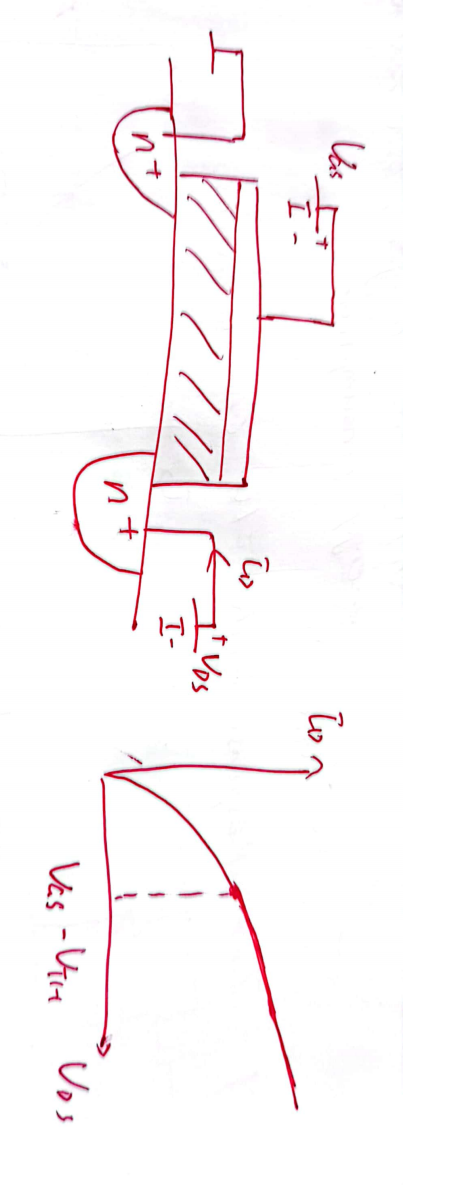
\includegraphics[scale=0.45]{1.jpg}}
    \captionsetup{labelformat=empty}
    \caption{}
    \label{1}
\end{figure}

As $V_{DS}\uparrow$, the Channel-Length $\downarrow$. 

Last day we didn't take this chagnge into consideration. Now let's rederive it. 
The upper limit of the integral on the left-hand side of the equation changes, leading to the increasing of $I_D$. 

$$\int_{0}^{L'} I_Ddx=\mu_{n}*W*C_{ox}*\int_{0}^{V_{GS}-V_{TH}} (V_{GS}-V_{TH}-V(x))dV$$

Actually, we can simply write down the conclusion with a correlation coefficient $\lambda$, showing the relationship between $V_{DS}$ and $I_D$ in pinch-off zone. 

$$I_D=\frac{1}{2} \mu C_{ox}\frac{W}{L}(V_{GS}-V_{TH})^2(1+\lambda V_{DS})$$

$\lambda$ (unit: $1/V$), is called the \textbf{Channel-Length Modulation Coefficient}. 

Then we can get a correct current source model. 

\begin{figure}[htbp]
    \centering
    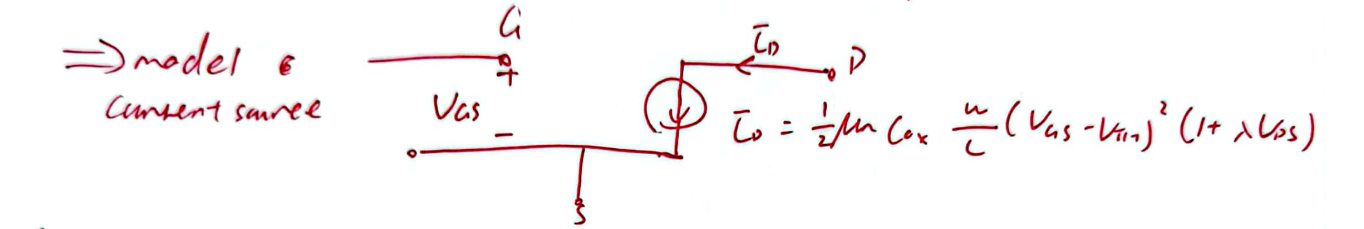
\includegraphics[scale=0.6]{2.jpg}
    \captionsetup{labelformat=empty}
    \caption{current source model with $\lambda$ taken into consideration}
    \label{2}
\end{figure}

\section*{Let's build an amplifer}

\textbf{Pay attention that we assume $\lambda=0$.} 

\begin{figure}[htbp]
    \centering
    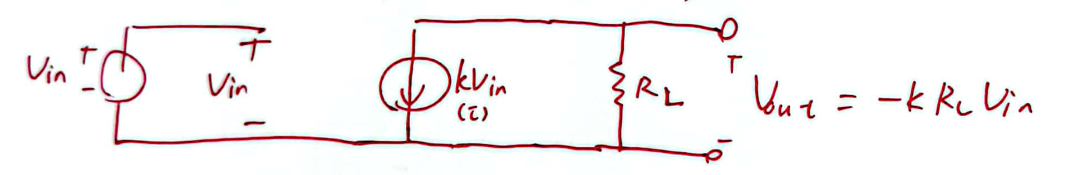
\includegraphics[scale=0.6]{3.jpg}
    \captionsetup{labelformat=empty}
    \caption{A simple amplifer model}
    \label{3}
\end{figure}

Assume that we hope to amplify a 5mV sound signal to 5V. 

\subsection*{First Attempt}

\begin{figure}[htbp]
    \centering
    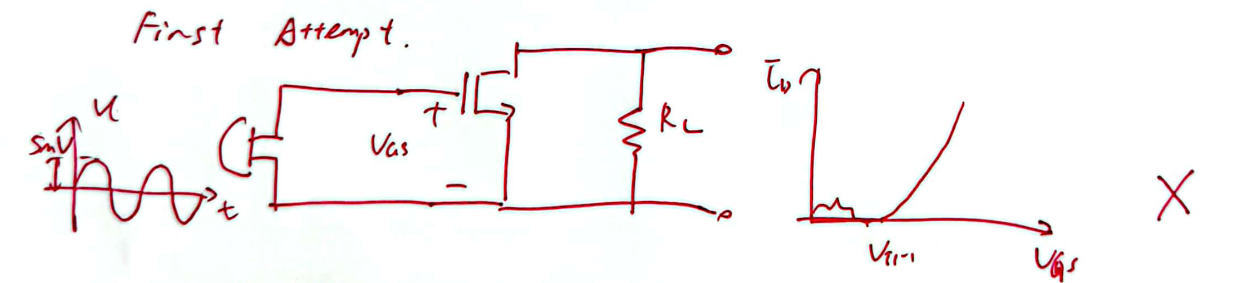
\includegraphics[scale=0.6]{4.jpg}
    \captionsetup{labelformat=empty}
    \caption{First attempt}
    \label{4}
\end{figure}

In this case we do not add a bias voltage. The MOSFET turns off. 

\subsection*{Second Attempt}

\begin{figure}[htbp]
    \centering
    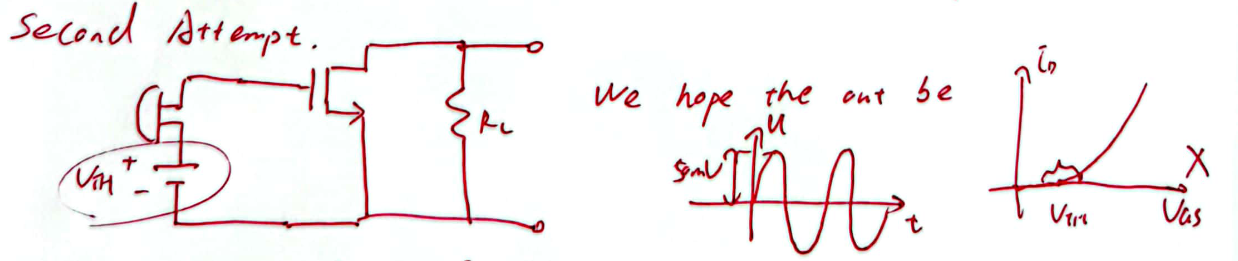
\includegraphics[scale=0.6]{5.jpg}
    \captionsetup{labelformat=empty}
    \caption{Second attempt}
    \label{5}
\end{figure}

In this case we add a bias voltage, we can calculate the $I_D$ after amplifering. 

Given that $\mu_nC_{ox}=100\mu A/V^2$, $\frac{W}{L}=10$, $V_{TH}=0.5V$. 

$$I_D=\frac{1}{2} \mu C_{ox}\frac{W}{L}(V_{GS}-V_{TH})^2=12.5nA$$

If we want the gain to be equal to 10, we need a resistor: 

$$R_L=\frac{50mV}{12.5nA}=4M\Omega$$

It's too large! Because the oprating point is close to $V_{TH}$, the gain is too small. 

\subsection*{Third Attempt}

\begin{figure}[htbp]
    \centering
    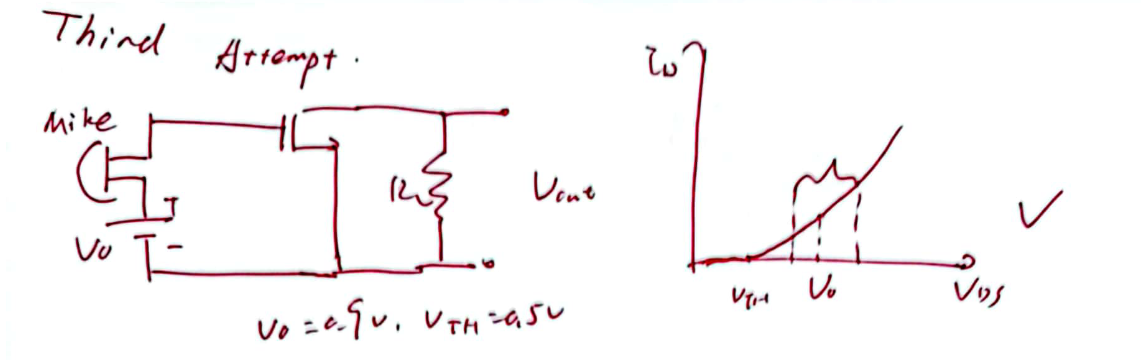
\includegraphics[scale=0.6]{6.jpg}
    \captionsetup{labelformat=empty}
    \caption{Third attempt}
    \label{6}
\end{figure}

We add a 0.9V bias to the Gate. This way we get a appropriate gain, a appropriate resistor. 

Let's calculate it. 

No signal: 

$$I_D=\frac{1}{2} \mu C_{ox}\frac{W}{L}(V_{GS}-V_{TH})^2=80\mu A$$

Max signal: 

$$I_D=\frac{1}{2} \mu C_{ox}\frac{W}{L}(V_{GS}-V_{TH})^2=82\mu A$$

The change in $I_D$ is $2\mu A$, we need a resistance $\frac{50mV}{2\mu A}=25k\Omega$. 

\subsection*{Conclusion}
\textbf{Need to bias the transistor by creating proper current and terminal voltage (in the absense of signals). 
So that the device can amplify the signal.}

However, $V_{DS}$ is not taken into consideration, it must make MOS enter the saturation zone. The model we create just now may not be correct enough. 
We'll talk about it next day. 

Today we only consider the \textbf{SATURATION} zone. 

\section*{Observation}

A MOS device "converts" a voltage to a current. With this ability we can call it a \textbf{Transconductor}. 

\begin{figure}[htbp]
    \centering
    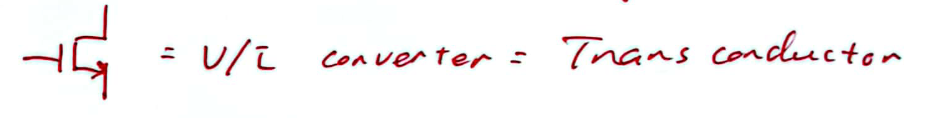
\includegraphics[scale=0.6]{7.jpg}
    \captionsetup{labelformat=empty}
    \caption{Transconductor}
    \label{7}
\end{figure}

Which operating point is preferred? 

\begin{figure}[htbp]
    \centering
    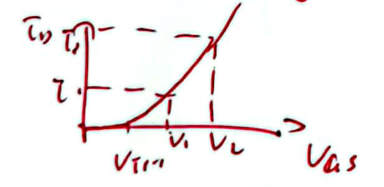
\includegraphics[scale=0.6]{8.jpg}
    \captionsetup{labelformat=empty}
    \caption{}
    \label{8}
\end{figure}

Actually, MOS operating in point 2 is stronger than point 1. But it consumes more energy because its drain current is larger. 

\section*{Combining Time Response with I/V Characteristics}

\begin{figure}[htbp]
    \centering
    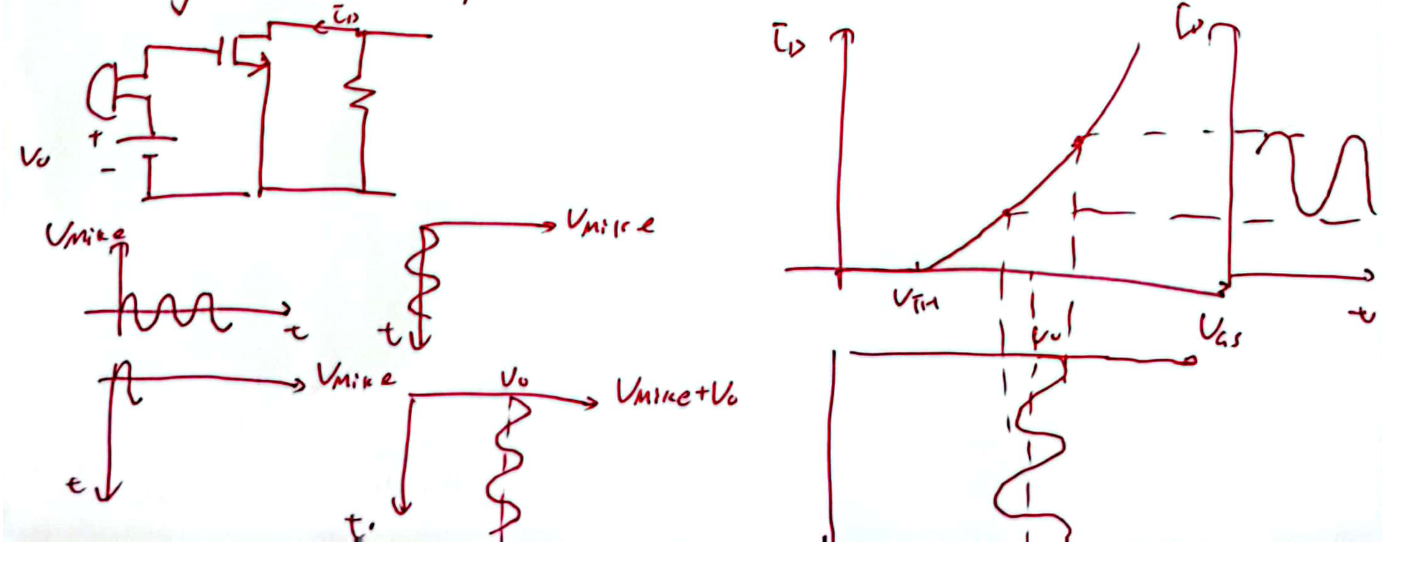
\includegraphics[scale=0.65]{9.jpg}
    \captionsetup{labelformat=empty}
    \caption{The relationship between $I_D$ and time}
    \label{9}
\end{figure}

Just rotate the voltage curve 90 degrees.

\section*{Concept of Transconductance}

We call the ability to convert a current into a voltage transconductance. 

$$g_m=\frac{dI_D}{dV_{GS}}$$

unit: $\frac{1}{\Omega}$, $S$, siemens. 

\begin{figure}[htbp]
    \centering
    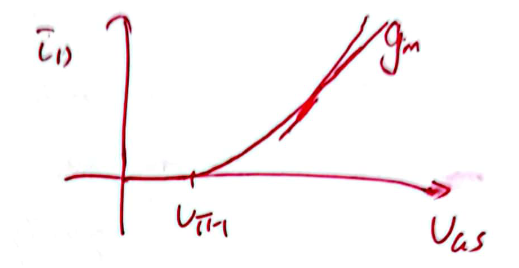
\includegraphics[scale=0.45]{10.jpg}
    \captionsetup{labelformat=empty}
    \caption{}
    \label{10}
\end{figure}

It represent on the graph as slope. 

\

From $I_D=\frac{1}{2} \mu C_{ox}\frac{W}{L}(V_{GS}-V_{TH})^2$, we can get: 

$$g_m=\frac{dI_D}{dV_{GS}}=\mu C_{ox}\frac{W}{L}(V_{GS}-V_{TH})$$

Or: 

$$g_m=\frac{2I_D}{V_{GS}-V_{TH}}$$

$$g_m=\sqrt{2I_D\mu C_{ox}\frac{W}{L}}$$

\section*{Link}

\href{https://www.bilibili.com/video/BV1FD4y1R7Ah?p=32&vd_source=1d0c07486a3bd3b0adb8ac548bf6453e}{Razavi Electronics Circuits 1: lectrue 32}
\end{document}